\documentclass[margin,line,a4paper,authoryear,12pt]{report}
\usepackage[utf8]{inputenc}%utf8
\usepackage[english]{babel}
\usepackage[T1]{fontenc}
\usepackage{graphicx,wrapfig}
\usepackage{url}
\usepackage{titlesec}
\usepackage[section]{placeins}
\usepackage{subcaption}

%\titleformat{\chapter}[display]
%    {\normalfont\bfseries}{}{0pt}{\Large}
\titleformat{\chapter}{\normalfont\huge}{\thechapter.}{20pt}{\huge\textbf}
\addtolength{\oddsidemargin}{-2cm}
\addtolength{\evensidemargin}{-2cm}
\addtolength{\textwidth}{4cm}
\addtolength{\topmargin}{-2cm}
\addtolength{\textheight}{4cm}



\begin{document}


\title{Advanced Software Engineering Documentation https://github.com/alexeifigueroa/ASEPetSynthesizer}
\author{Alexei Figueroa}
\date{February 2018}
\maketitle

\tableofcontents
%======================================================================================================================================
\chapter{Introduction}
This documentation highlights the implementation of the techniques 
provided in the Advanced Software Engineering lecture. The aplication developed
consists of a simple piano developed using the \texttt{Python} language with the help
of the libraries \texttt{pygame} and \texttt{scipy}. The main paradigm behind the
architecture of the application is the Model View Presenter, relaxations are made
to cover as much as possible the requirements of the assignment. The mechanism of generation of the sound is based on the model of an
analog synthesizer. Several simplifications are made to limit the complexity of the software. The synthesizer accepts only keyboard input, 
it requires an audio device and it has been tested on ubuntu 17.10 and Windows 10 and minimally in the trusty environment of TravisCI.
\begin{figure}[h!]
    \centering
    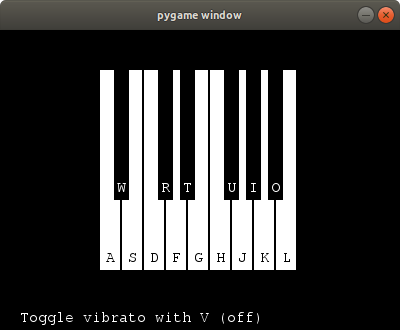
\includegraphics[width=0.6\linewidth]{Synthesizer.png}
    \caption{GUI of the synthesizer}
    \label{fig:synthesizer}
\end{figure}    
%======================================================================================================================================
\chapter{UML}
\section{Class Diagram}
    \begin{figure}[h!]
        \centering
        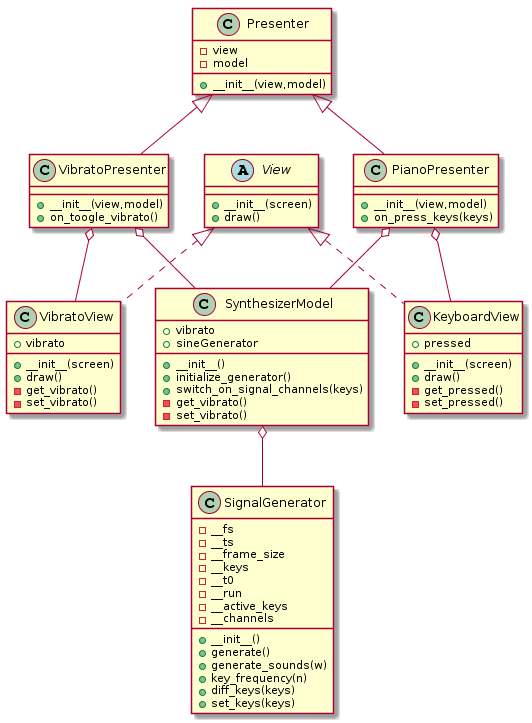
\includegraphics[width=0.6\linewidth]{UML/ClassDiagram.png}
        \caption{Class Diagram of the synthesizer}
        \label{fig:ClassDiagram}
    \end{figure} 
\section{Sequence Diagram}
    \begin{figure}[h!]
        \centering
        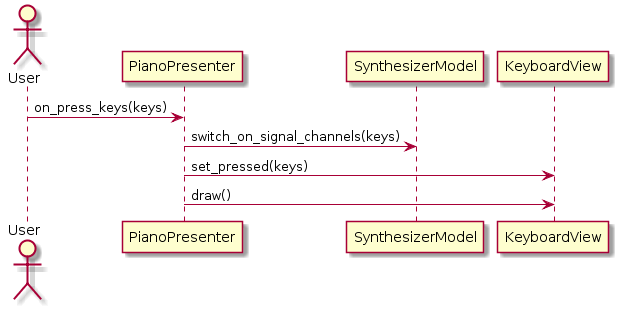
\includegraphics[width=0.8\linewidth]{UML/SequenceDiagram.png}
        \caption{Sequence Diagram of the synthesizer describing the MVP calls given a user key event.}
        \label{fig:SequenceDiagram}
    \end{figure}
\section{State Diagram}
\begin{figure}[h!]
    \centering
    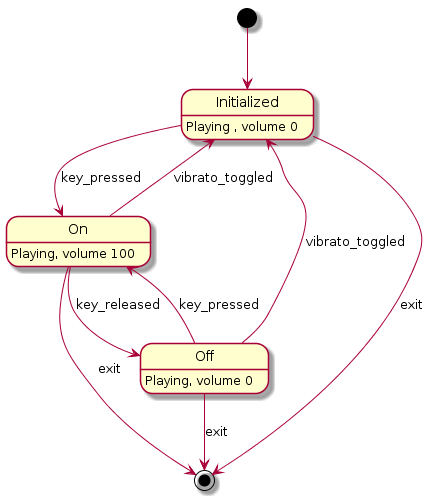
\includegraphics[width=0.5\linewidth]{UML/StateDiagram.png}
    \caption{State Diagram of a mixer channel}
    \label{fig:StateDiagram}
\end{figure}
\section{Activity Diagram}
\begin{figure}[h!]
    \centering
    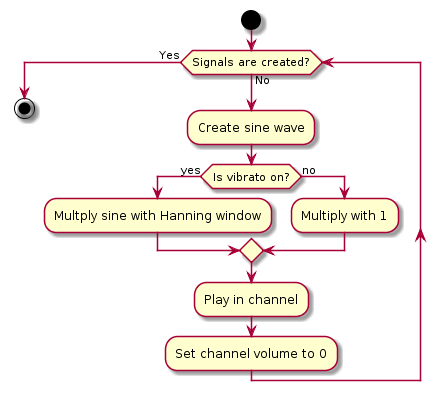
\includegraphics[width=0.5\linewidth]{UML/ActivityDiagram.png}
    \caption{Activity Diagram describing the sound generation for all channels.}
    \label{fig:ActivityDiagram}
\end{figure}
\section{Object Diagram}
\begin{figure}[h!]
    \centering
    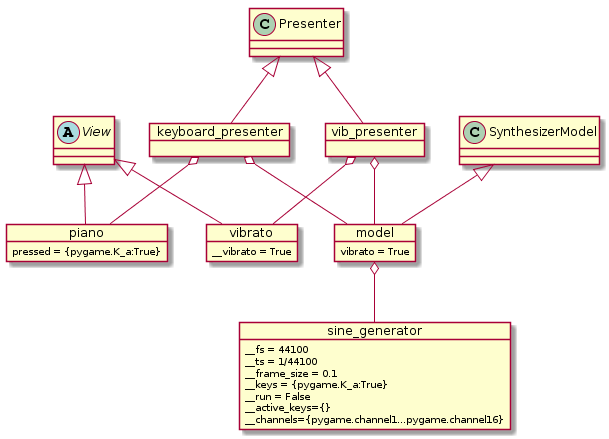
\includegraphics[width=0.8\linewidth]{UML/ObjectDiagram.png}
    \caption{Object Diagram of key "A" pressed with the vibrato turned on, additionally the Views, Presenters and Model are indicated.}
    \label{fig:ObjectDiagram}
\end{figure}
%======================================================================================================================================
\chapter{Metrics}
The SonarCloud platform was chosen to run the code analysis on the code, The project metrics can be accessed through
\url{https://sonarcloud.io/organizations/alexeifigueroa-github/projects}

\begin{figure}[h!]
    \centering
    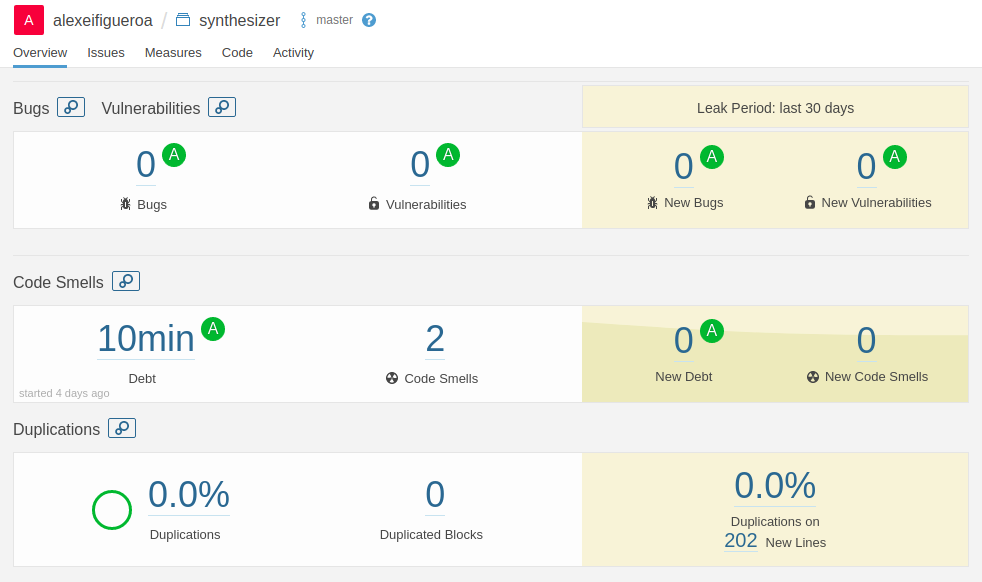
\includegraphics[width=0.8\linewidth]{SonarCloud.png}
    \caption{Dashboard of SonarCloud of the project}
    \label{fig:SonarCloud}
\end{figure}

\begin{figure}[h!]
    \begin{subfigure}{0.4\linewidth}
    \centering
    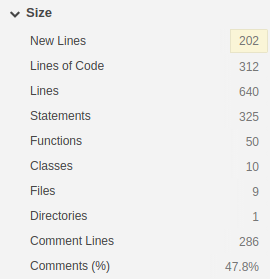
\includegraphics[width=\linewidth]{Size_measures.png}
    \caption{Size measures}
    \label{fig:SonarCloud}
    \end{subfigure}
    \begin{subfigure}{0.4\linewidth}
        \centering
        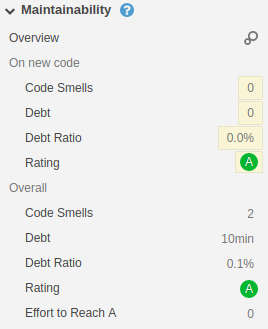
\includegraphics[width=\linewidth]{maintainability_measures.png}
        \caption{Maintainability measures. }
        \label{fig:SonarCloud}
    \end{subfigure}
    \\
    \begin{subfigure}{\linewidth}
        \centering
        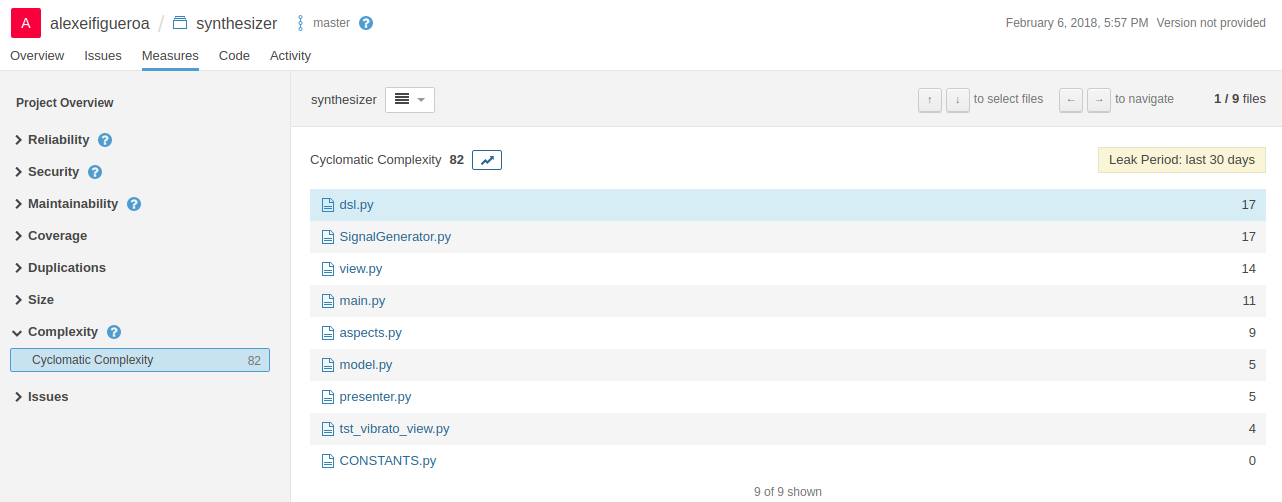
\includegraphics[width=\linewidth]{cyclomatic_complexity.png}
        \caption{Cyclomatic complexity. }
        \label{fig:SonarCloud}
    \end{subfigure}
    \caption{Metrics of SonarCloud for the synthesizer project.}
\end{figure}

%======================================================================================================================================
\chapter{Clean Code Development}
\section{Version Control}
Since it's inception this project was developed using git as the version control system with the repository being hosted on github.
\begin{figure}[h!]
    \centering
    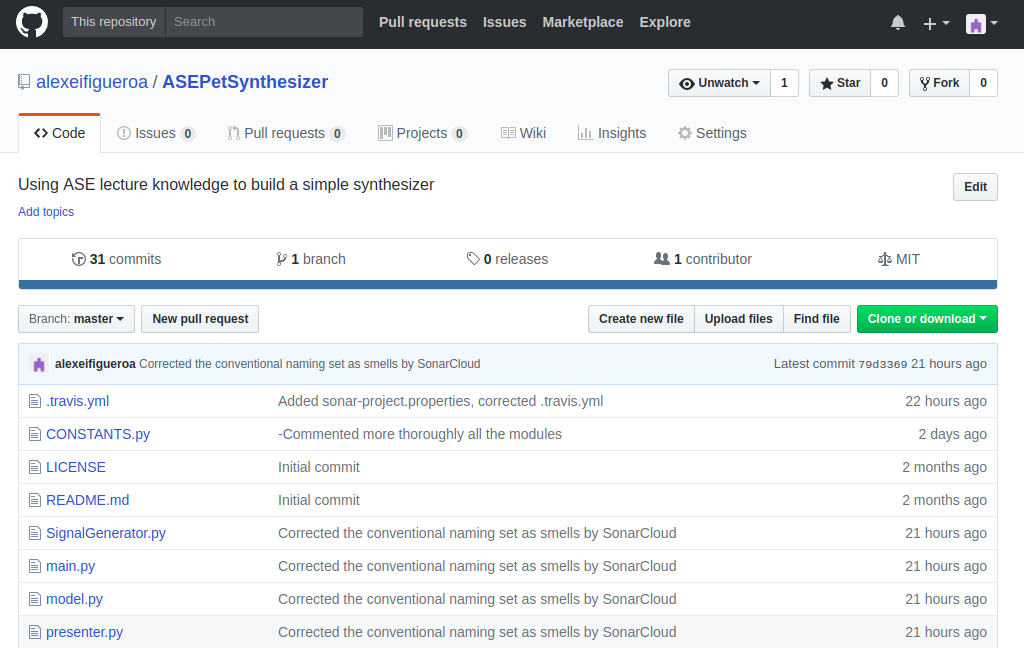
\includegraphics[width=0.8\linewidth]{github.png}
    \caption{Github repository main page}
    \label{fig:github}
\end{figure}
\begin{figure}[h!]
    \centering
    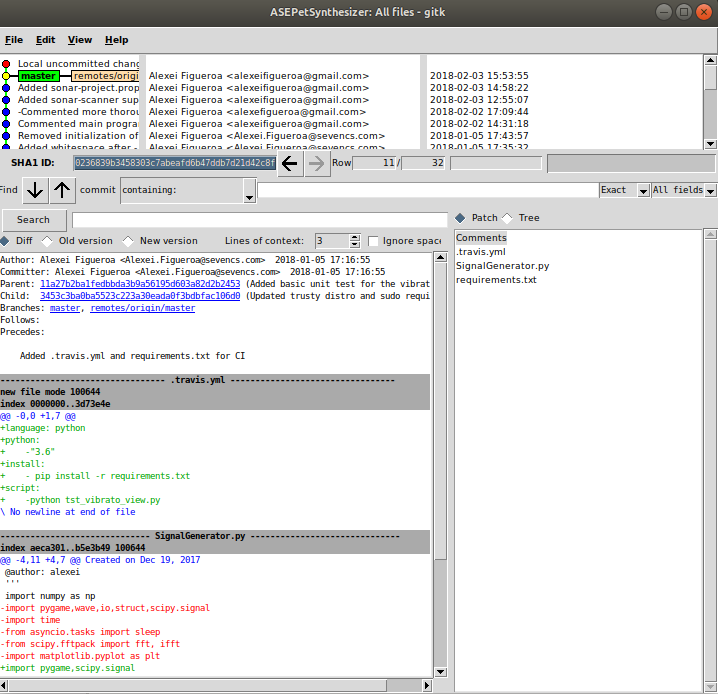
\includegraphics[width=0.8\linewidth]{gitk.png}
    \caption{Gitk frontend on development machine}
    \label{fig:gitk}
\end{figure}
\section{Continuous Integration}
TravisCI was the platform of choice for orchestrating the building,testing and triggering the code analysis by SonarCloud. The .travis.yml file is under the root of the repository,
after providing TravisCI access to the Github account, as soon as a git push is through the whole process is run.
\begin{figure}[h!]
    \centering
    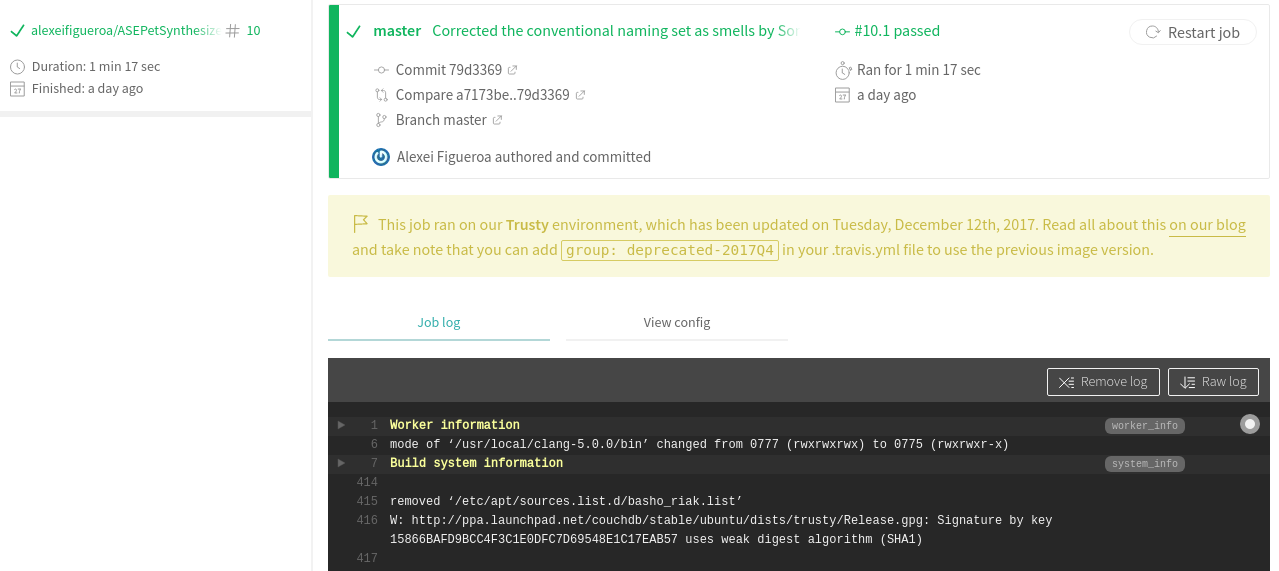
\includegraphics[width=\linewidth]{travis_build_log.png}
    \caption{TravisCI, build log after a succesful run.}
    \label{fig:travisRun}
\end{figure}

\section{Architecture and class design, separation of concerns\cite{CleanCodeBook}}
The purpose of the program presented in this work is to simulate an analogue synthesizer. Such hardware is normally conceived as a
modular device by itself, composed out of smaller very domain specific tools. The intricate domain logic makes a software simulation
naturally exploit the abstraction and isolation of concerns. A fair methodology to achieve this is the Model View Presenter architecture 
which splits the domain logic into a \textbf{Model}, the user interactive functionality into a \textbf{View} and the presentational logic which integrates 
it all in a \textbf{Presenter}. In this work the \textbf{Model} logic is implemented into a single class which aggregates a SignalGenerator. Further
domain specific hardware that was not implemented in this project, like for instance a voltage controlled filter VCO could be integrated here.
Additionally the Views representing a piano Keyboard and a vibrato switch were implemented. Finally the Presenter module synchronizes the interaction
of the user by triggering the event handlers and modifying the \textbf{Model} and the \textbf{View} accordingly.
\begin{figure}[h!]
    \centering
    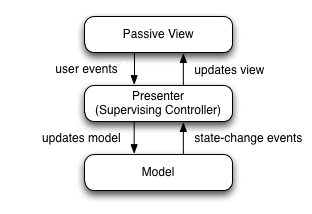
\includegraphics[width=0.5\linewidth]{MVP.png}
    \caption{Diagram representing the MVP design pattern\cite{MVP}.}
    \label{fig:MVP}
\end{figure}

\section{Automated Unit Tests}
The choice in architecture of the program presented is well suited for unit testing. The library chosen for such tests is the default
standard unittest library shipping with the Python interpreter. A model test for the View of the vibrato control is shown next. These unit test
is executed at the end of the build process by the CI environment.
\begin{figure}[h!]
    \centering
    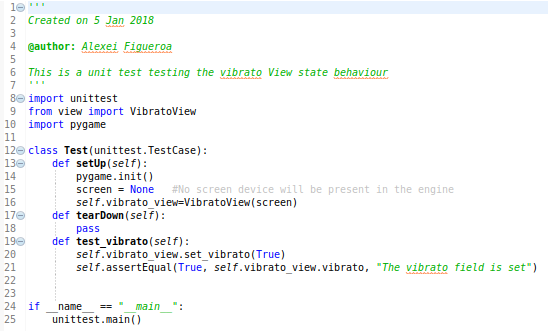
\includegraphics[width=0.8\linewidth]{vibrato_test.png}
    \caption{Snipet of tst\_vibrato\_view.py}
    \label{fig:gitk}
\end{figure}
\section{Source Code conventions}
The usage of source code conventions was checked mainly with the assistance of SonarCloud, a good example are the naming conventions.
The following figure highlights 3 different examples, it's important to know that for the 2 last ones, setUp and tearDown methods, these names
are part of a mandatory interface specification of the unittest Python standard library.
\begin{figure}[h!]
    \centering
    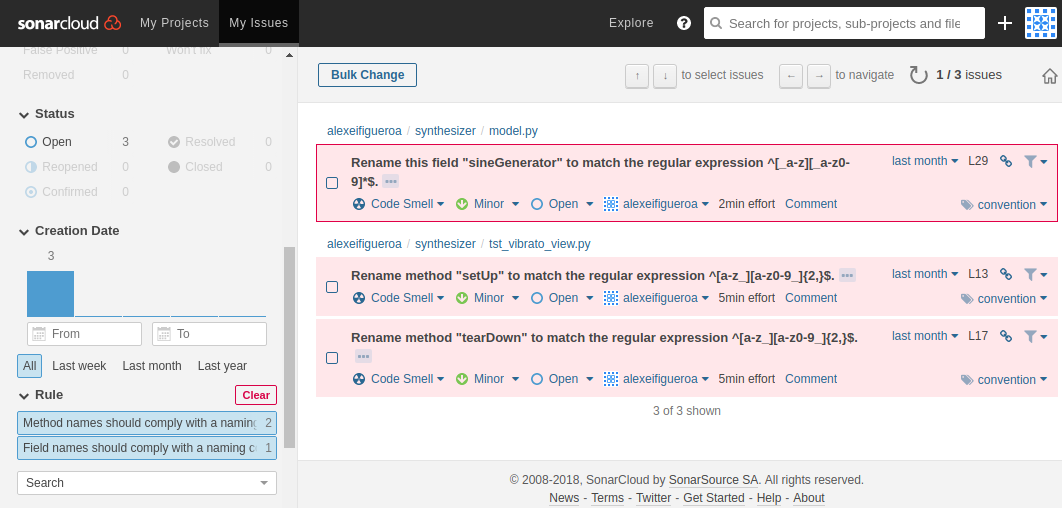
\includegraphics[width=\linewidth]{naming_convention.png}
    \caption{Sonar Cloud "smells" pointing at naming convention failures}
    \label{fig:smells}
\end{figure}


\section{Static Code Analysis}

As mentioned before the SonarCloud platform was used for the code analysis. Some of the size metrics are depicted next.

\begin{figure}[h!]
    \centering
    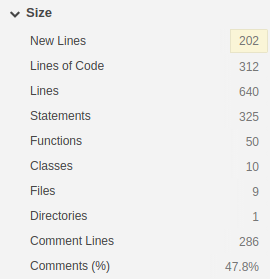
\includegraphics[width=0.4\linewidth]{Size_measures.png}
    \caption{Sonar Cloud Size metrics for the project.}
    \label{fig:smells}
\end{figure}

%======================================================================================================================================
\chapter{Continuous Delivery}
As mentioned before, the system for Continuous Integration chosen was TravisCI.
The build history and contents of the .travis.yml file can be seen next.
\begin{figure}[h!]
    \centering
    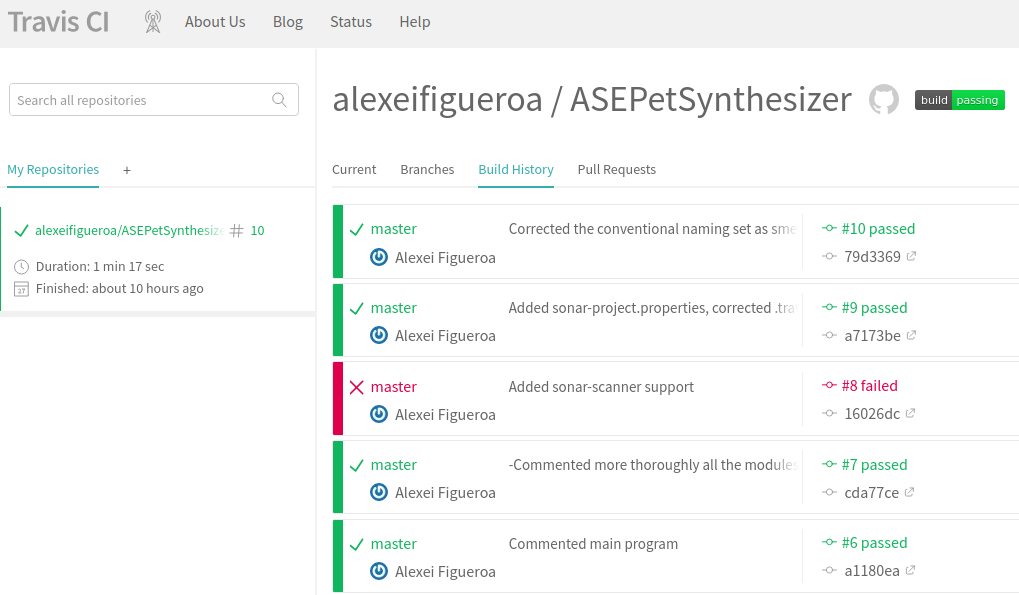
\includegraphics[width=0.8\linewidth]{TravisCI.png}
    \caption{Build history in Travis-CI}
    \label{fig:TravisCI}
\end{figure}
\begin{figure}[h!]
    \centering
    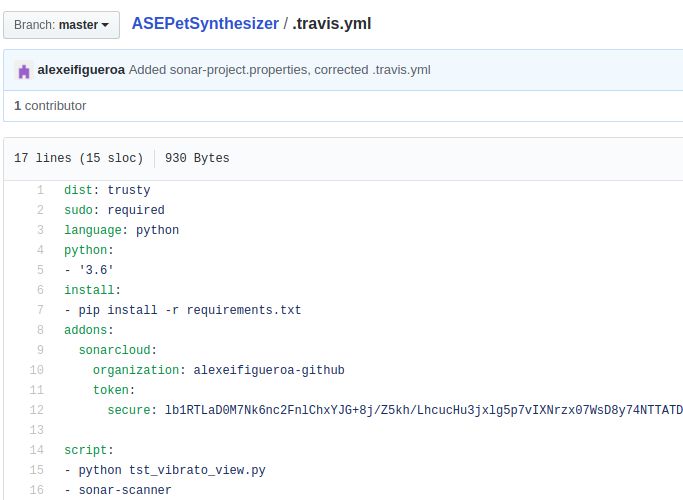
\includegraphics[width=0.8\linewidth]{travis_yml.png}
    \caption{Contents of .travis.yml}
    \label{fig:TravisCI}
\end{figure}
%======================================================================================================================================
\chapter{AOP}

Aspect Oriented Programming in the context of this work is applied by 
the means of python decorators, these are high order functions that 
wrap their arguments with code placed before and after the function of interest.
This function can be optionally executed. For the purposes of the synthesizer 
simulation a critical operation is the responsiveness of the program to react to the
user pressing a key. Following this ideas the event handler for any key press is logged
to expose the keys that are pressed (in case of multiplicity), and timed. This is implemented in the PianoPresenter class with non invasive code
by the means of the \texttt{@decorator} notation. 
The implementation of both wrappers is under the aspects module.
\begin{figure}[h!]
    \centering
    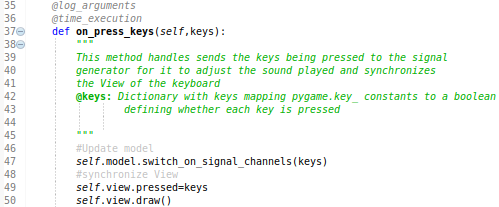
\includegraphics[width=0.8\linewidth]{Piano_presenter_event.png}
    \caption{ Decorators placed around the key pressing event handler.}
    \label{fig:aspects}
\end{figure}

\begin{figure}[h!]
    \centering
    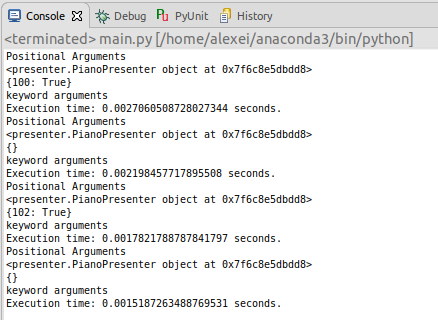
\includegraphics[width=0.8\linewidth]{PianoPresenter_log_time.png}
    \caption{Logging of keys and execution times at runtime for both key pressing and releasing of two distinct keys.}
    \label{fig:aspects}
\end{figure}

\begin{figure}[h!]
    \centering
    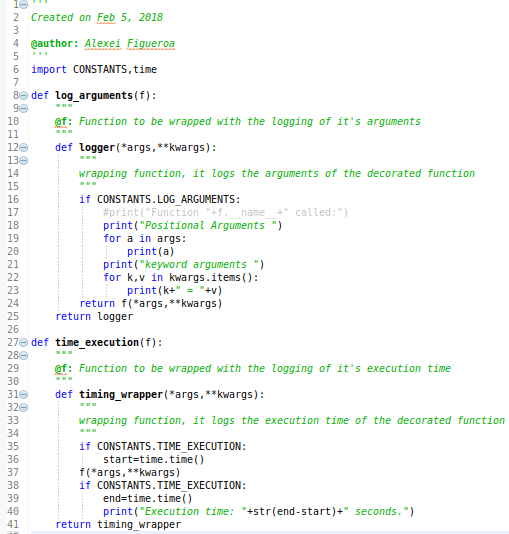
\includegraphics[width=0.8\linewidth]{AOP_wrappers.png}
    \caption{ Higher order functions for execution timing and logging arguments in the aspects.py module}
    \label{fig:aspects}
\end{figure}


%======================================================================================================================================
\chapter{DSL}

An analogue synthesizer comprehends a signal processing pipeline. Signals from a signal generator are added, and subsequently transformed 
to an output that is converted to audio. The DSL proposed with this project is for purposes of describing the pipeline of 
audio synthesizer. Deliberately 2 different approaches where implemented to describe this tipe of pipeline: an object oriented class implementing
chaining of the transformation of it's sole attribute (a signal), and a functional approach describing a composition of functions. These
are located under the \texttt{dsl} module and demo applications are presented next.
\begin{figure}[h!]
    \centering
    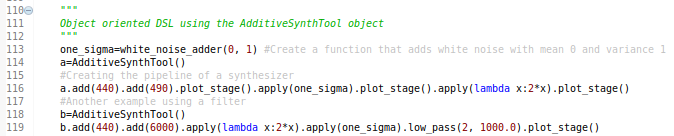
\includegraphics[width=\linewidth]{dsl_oop_example.png}
    \caption{ Object oriented functionality of building a signal transformation pipeline.}
    \label{fig:dsl_oop}
\end{figure}

\begin{figure}[h!]
    \begin{subfigure}{0.3\linewidth}
        \centering
        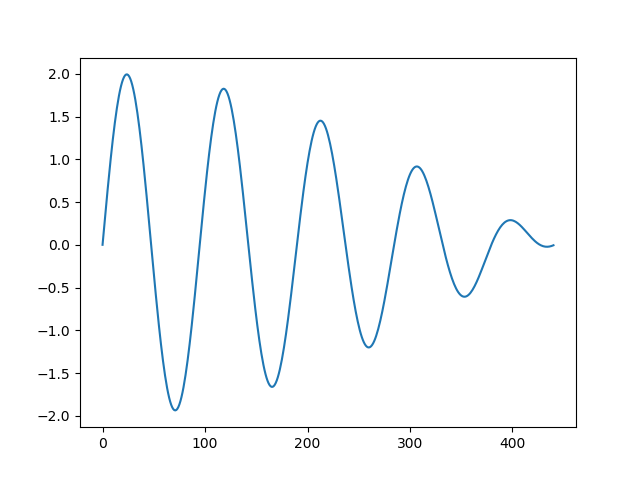
\includegraphics[width=\linewidth]{oop_two_sines.png}
        \caption{First plot\_stage call, only 2 sine waves in the pipeline}
        \label{fig:SonarCloud}
    \end{subfigure}
    \begin{subfigure}{0.3\linewidth}
        \centering
        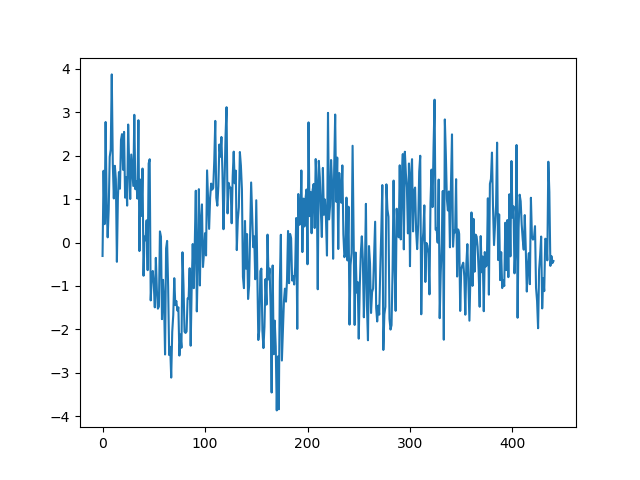
\includegraphics[width=\linewidth]{oop_two_sines_noise.png}
        \caption{Second plot\_stage call, white noise is added to the pipeline }
        \label{fig:SonarCloud}
    \end{subfigure}
    \begin{subfigure}{0.3\linewidth}
        \centering
        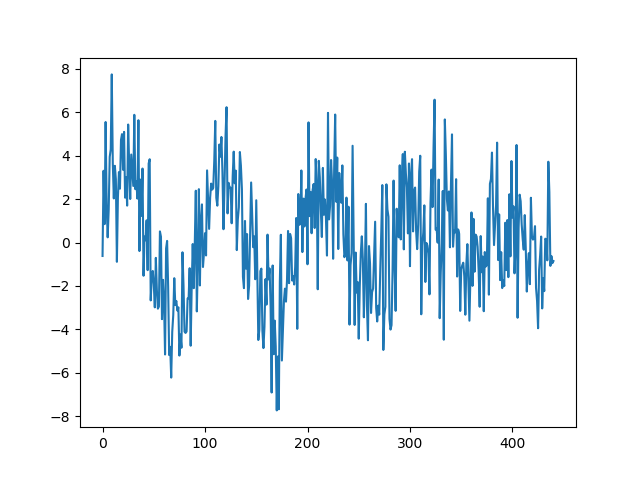
\includegraphics[width=\linewidth]{oop_two_sines_noise_times_2.png}
        \caption{Third plot\_stage call,the signal is doubled  }
        \label{fig:SonarCloud}
    \end{subfigure}
    \caption{Execution of line 116 plotting the signal at different stages of the transformation pipeline}
\end{figure}

The class that makes the chaining of the pipeline possible is presented next, followed by the functions and Closures for the functional programming approach.
\begin{figure}[h!]
    \centering
    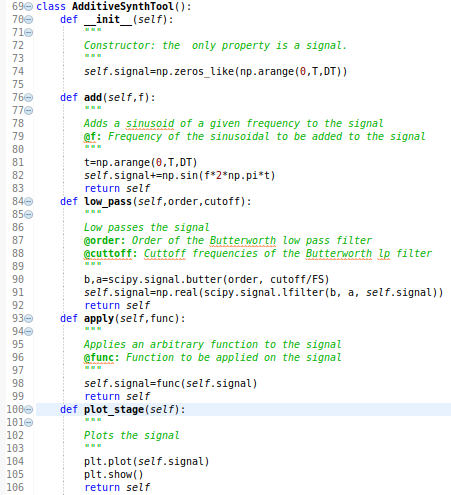
\includegraphics[width=0.8\linewidth]{dsl_class_snippet.png}
    \caption{ Class to generate signals by providing methods that can be chained in the object oriented DSL.}
    \label{fig:dsl_class}
\end{figure}

\begin{figure}[h!]
    \centering
    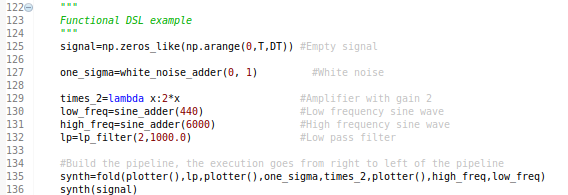
\includegraphics[width=\linewidth]{dsl_functional_example.png}
    \caption{ Functional approach of building a signal transformation pipeline.}
    \label{fig:dsl_oop}
\end{figure}

\begin{figure}[h!]
    \begin{subfigure}{0.3\linewidth}
        \centering
        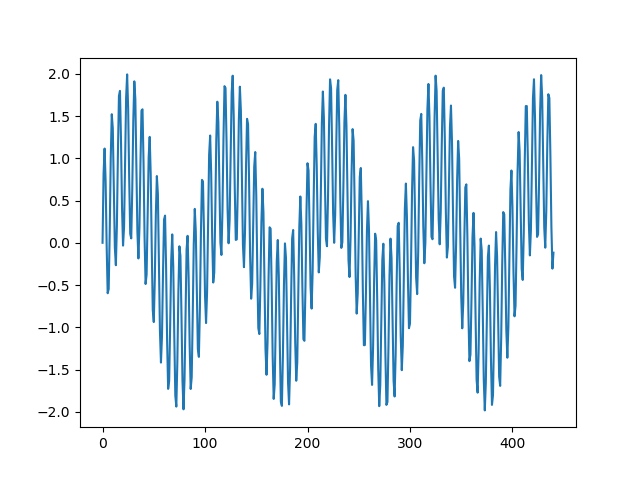
\includegraphics[width=\linewidth]{func_2_sines.png}
        \caption{First plotter() closure , only 2 sine waves in the pipeline}
        \label{fig:SonarCloud}
    \end{subfigure}
    \begin{subfigure}{0.3\linewidth}
        \centering
        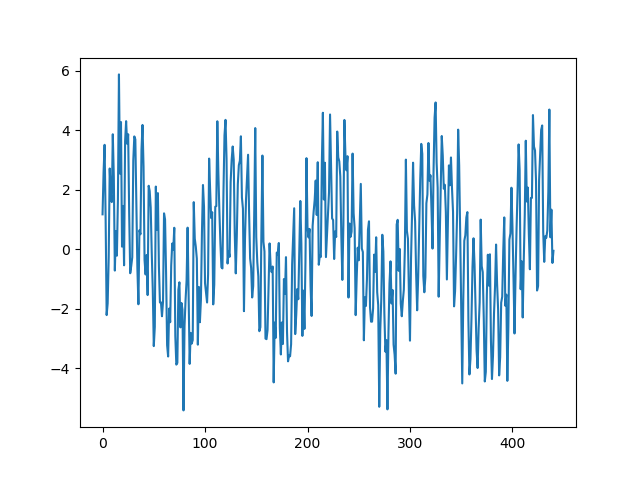
\includegraphics[width=\linewidth]{func_2_sines_noise.png}
        \caption{Second plotter() closure , white noise is added to the pipeline }
        \label{fig:SonarCloud}
    \end{subfigure}
    \begin{subfigure}{0.3\linewidth}
        \centering
        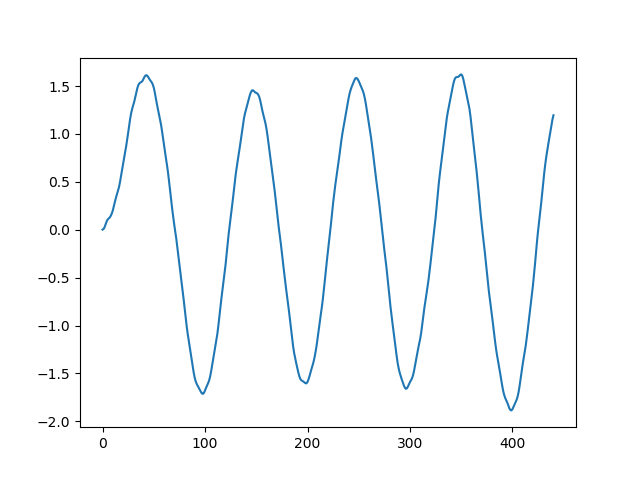
\includegraphics[width=\linewidth]{func_2_sines_noise_filtered.png}
        \caption{Third plotter() closure ,the signal is filtered for one sinewave and the noise }
        \label{fig:SonarCloud}
    \end{subfigure}
    \caption{Execution of line 135,136 plotting the signal at different stages of the transformation pipeline using functional programming only.}
\end{figure}



\begin{figure}[h!]
    \centering
    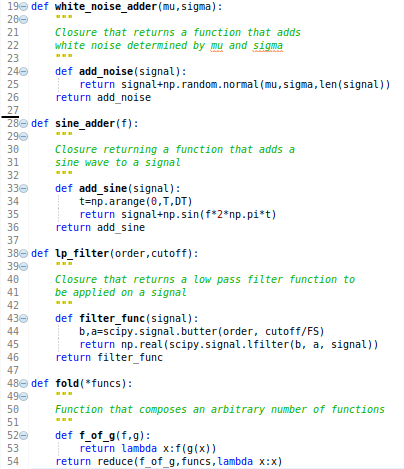
\includegraphics[width=0.7\linewidth]{dsl_closures.png}
    \caption{ Closures and functions needed to transform an input signal in the functional programming DSL.}
    \label{fig:dsl_class}
\end{figure}
%======================================================================================================================================
\chapter{Functional Programming}
Although the architecture for the development of this project was chosen to be MVP, hence
object oriented. The following concepts of functional programming were applied as strictly as possible.
\section{Final data structures}
Python is not a purely functional programming language ,nevertheless the 
practice of only having final data structures can be achieved by keeping them unmodified : 
never at the left of the assignment operator\cite{pythonFunctional}.

\section{Side effect free functions}
Since the application is purported for sound device output, these side effects
are relaxed and thus allowed in the functions. Next figure depicts the extent of what is probably the most
complex function in the project. The side effects: only related ot the audio stream are highlighted.
\begin{figure}[h!]
    \centering
    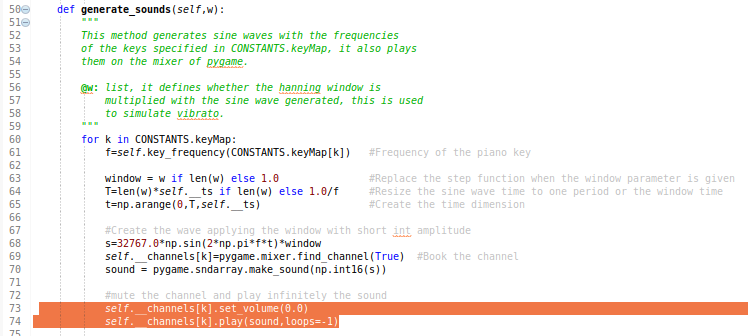
\includegraphics[width=\linewidth]{Side_effects.png}
    \caption{ method generate\_sounds from the class SignalGenerator, the side effects are highlighted.}
    \label{fig:aspects}
\end{figure}
\section{Higher order functions, functions as parameters and return values}
As explained above the Aspect Oriented functionality was implemented by the use of decorators, which
are indeed higher order functions. Furthermore they receive functions as parameters and also return
functions. Additionally the closures developed for the DSL presented in the  next session also present this behaviour.
\begin{figure}[h!]
    \centering
    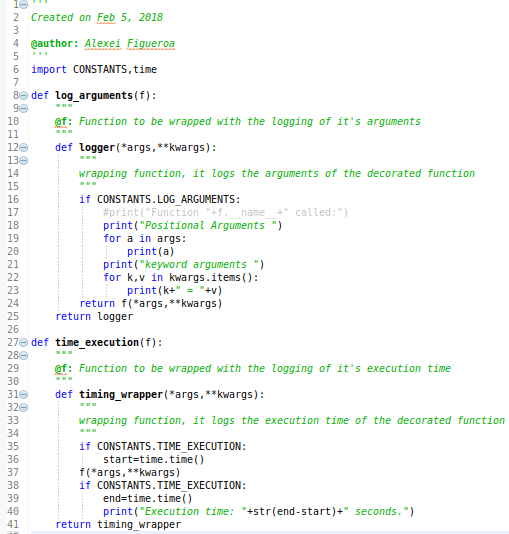
\includegraphics[width=0.8\linewidth]{AOP_wrappers.png}
    \caption{ Higher order functions for execution timing and logging arguments in the aspects.py module}
    \label{fig:aspects}
\end{figure}
\section{Closures / anonymous functions}
As mentioned in the DSL chapter, several closuers were developed to achieve a functionally composed pipeline
of sound generation, aditionally lambdas (anonymous functions) were used for both the purposes of composition
of functions as well as creating signal transformations (\texttt{lambda x:2*x} doubles a signal amplitude).
\begin{figure}[h!]
    \centering
    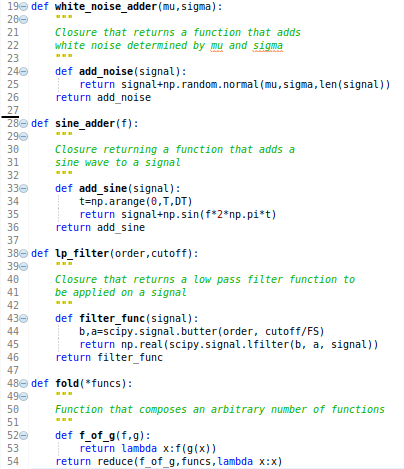
\includegraphics[width=0.7\linewidth]{dsl_closures.png}
    \caption{ Closures and functions needed to transform an input signal in the dsl module.}
    \label{fig:dsl_class}
\end{figure}


%======================================================================================================================================
\chapter{Logical solver}
The control of the audio output of the program as previously depicted in the state diagram of an individual audio channel is
mainly done by switching the volume on or off, for this to happen at each event of a key press, a check is made to see whether the
keys pressed are different and then if so, all the channels are switched off and the corresponding active channels are turned on. 

 
\begin{center}
    \begin{figure}[h!]
        \begin{subfigure}{0.8\linewidth}
            \centering
            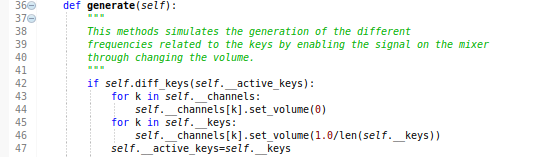
\includegraphics[width=\linewidth]{SignalGenerator_generate.png}
            \caption{\texttt{generate} method of the \texttt{SignalGenerator class}}
            \label{fig:generate}
        \end{subfigure}
        \begin{subfigure}{0.8\linewidth}
            \centering
            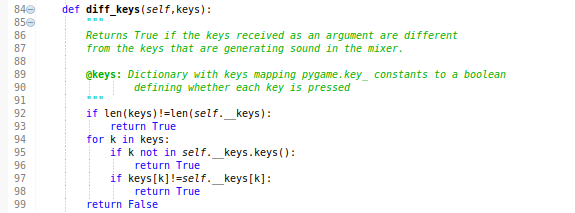
\includegraphics[width=\linewidth]{SignalGenerator_diff_keys.png}
            \caption{\texttt{diff\_keys} method of the \texttt{SignalGenerator class}}
            \label{fig:diffkeys}
        \end{subfigure}
        
        \caption{Methods from the SignalGenerator class that control the logic behind the swiching on and off of the audio channels}
    \end{figure}
\end{center}

A way of optimizing this implementation would be to selectively turn on or off the channels that are different between the two 
distinct points in time and such very simple scenario could be approached by a logical solver.  In the following example are shown
in \texttt{prolog} the definition of the facts and rules for any arbitrary two time steps (key events) ,as well as the  queries that would give 
full information of what channels to turn on or off. 
\begin{figure}[h!]
    \centering
    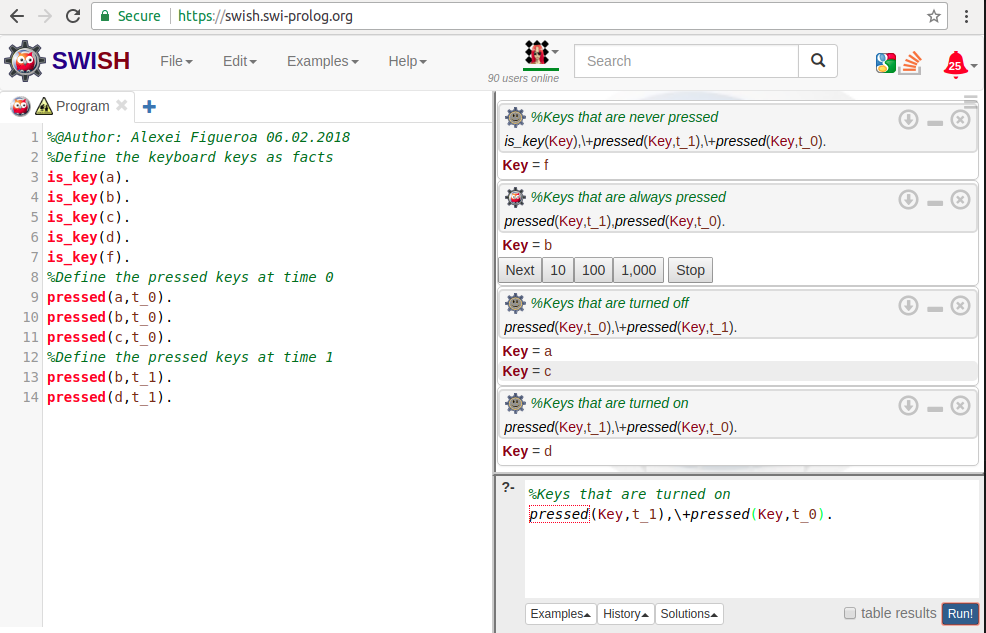
\includegraphics[width=\linewidth]{prolog_solved_expressions.png}
    \caption{ Prolog simple model solution to "diff" the channels to activate/deactivate given an key event.}
    \label{fig:prolog}
\end{figure}
%======================================================================================================================================
\chapter{Code fragment in Scala}
A small fragment of code computing the mean of a set of 100 standard normally distributed random numbers is depicted next.
\begin{figure}[h!]
    \centering
    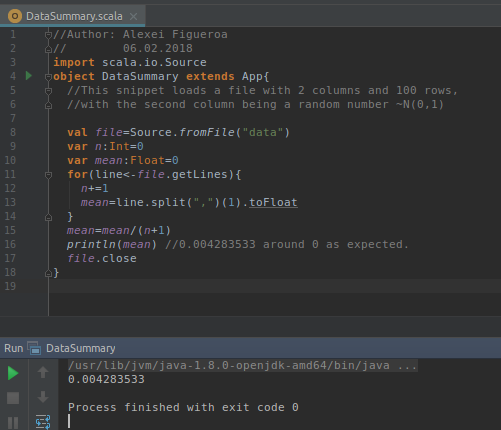
\includegraphics[width=0.7\linewidth]{scala.png}
    \caption{ Scala code snippet that reads a csv and computes the mean of the 2nd column.}
    \label{fig:dsl_class}
\end{figure}

\begin{thebibliography}{9}

\bibitem{CleanCodeBook}
Cleancodedeveloper.com,\textit{Clean Code Developer: Virtues}\\
\texttt{https://ccd\_school.gitbooks.io/clean-code-developer-com/content/\\01abstractions/03\_Virtues.html}\\visited on 21.12.2017 

\bibitem{MVP}
Wikipedia,\textit{Model View Presenter}\\
\texttt{https://en.wikipedia.org/wiki/Model-view-presenter}\\
visited on 21.12.2017 

\bibitem{pythonFunctional}
A.M.Kuchling,\textit{Functional Programing HOWTO}\\
\texttt{https://docs.python.org/3.6/howto/functional.html}\\
visited on 21.12.2017 


\bibitem{synthesizer}
Wikipedia,\textit{Synthesizer}\\
\texttt{https://en.wikipedia.org/wiki/Synthesizer}
visited on 21.12.2017

\bibitem{GUIArch}
M. Fowler, \textit{GUI Architectures}\\
\texttt{https://www.martinfowler.com/eaaDev/uiArchs.html}
visited on 20.09.2017
\bibitem{PassiveView}
M. Fowler\textit{Passive View}\\
\texttt{https://martinfowler.com/eaaDev/PassiveScreen.html}\\
visited on 20.09.2017
\end{thebibliography}

\end{document}